\documentclass{standalone}
\usepackage{tikz}
\begin{document}

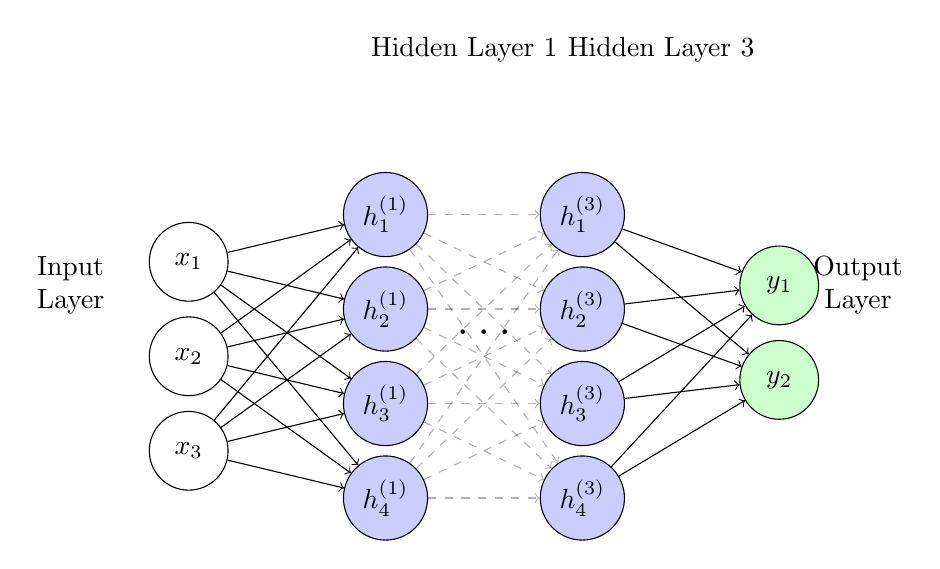
\begin{tikzpicture}

    % Define layer and node spacing
    \def\layersep{2.5} % distance between layers
    \def\nodesep{1.2}  % vertical space between nodes

    % Input layer
    \foreach \i in {1, 2, 3}
        \node[circle, draw, minimum size=1cm] (I-\i) at (0,-\i*\nodesep) {$x_{\i}$};

    % First hidden layer
    \foreach \i in {1, 2, 3, 4}
        \node[circle, draw, fill=blue!20, minimum size=1cm] (H1-\i) at (\layersep,-\i*\nodesep+0.6) {$h^{(1)}_{\i}$};

    % Second hidden layer (represented by dots)
    \node at (1.5*\layersep, -2*\nodesep+0.3) {\LARGE $\ldots$};

    % Third hidden layer
    \foreach \i in {1, 2, 3, 4}
        \node[circle, draw, fill=blue!20, minimum size=1cm] (H3-\i) at (2*\layersep,-\i*\nodesep+0.6) {$h^{(3)}_{\i}$};

    % Output layer
    \foreach \i in {1, 2}
        \node[circle, draw, fill=green!20, minimum size=1cm] (O-\i) at (3*\layersep,-\i*\nodesep-0.3) {$y_{\i}$};

    % Draw connections between Input and First Hidden layer
    \foreach \i in {1, 2, 3}
        \foreach \j in {1, 2, 3, 4}
            \draw[->] (I-\i) -- (H1-\j);

    % Draw faded, dashed connections between First and Third Hidden layers
    \foreach \i in {1, 2, 3, 4}
        \foreach \j in {1, 2, 3, 4}
            \draw[->, dashed, opacity=0.3] (H1-\i) -- (H3-\j);

    % Draw connections between Third Hidden and Output layers
    \foreach \i in {1, 2, 3, 4}
        \foreach \j in {1, 2}
            \draw[->] (H3-\i) -- (O-\j);

    % Labels for layers
    \node[align=center] at (-1.5, -1.5) {Input \\ Layer};
    \node[align=center] at (\layersep+1, 1.5) {Hidden Layer 1};
    \node[align=center] at (2*\layersep+1, 1.5) {Hidden Layer 3};
    \node[align=center] at (3*\layersep+1, -1.5) {Output \\ Layer};

\end{tikzpicture}

\end{document}
